\documentclass[12pt,a4paper]{article}

\usepackage[utf8]{inputenc}
\usepackage[T1]{fontenc}
\usepackage{lmodern}
\usepackage[a4paper,margin=2.5cm]{geometry}
\usepackage{amsmath,amssymb,mathtools}
\usepackage{booktabs,longtable,array,tabularx}
\usepackage{graphicx}
\usepackage{xcolor}
\usepackage{enumitem}
\usepackage{setspace}
\usepackage{authblk}
\usepackage[numbers,sort&compress]{natbib}
\usepackage{hyperref}
\usepackage{fancyhdr}
\usepackage{titlesec}
\usepackage{listings}
\usepackage{siunitx}
\sisetup{group-separator={,}, group-minimum-digits=4}
% \day and \month are LaTeX date counters and clash with siunitx unit parsing;
% declare non-clashing macros instead of overloading them.
\DeclareSIUnit{\dday}{day}
\DeclareSIUnit{\dmonth}{month}

\newcommand{\E}{\mathbb{E}}
\newcommand{\R}{\mathbb{R}}
\newcommand{\dif}{\,\mathrm{d}}

\definecolor{mosblue}{HTML}{1F4E79}
\definecolor{mosgreen}{HTML}{1D7A5A}
\definecolor{mosorange}{HTML}{C77700}
\definecolor{lightgray}{HTML}{F4F6F7}
\definecolor{darkred}{HTML}{8B1A1A}

\hypersetup{colorlinks=true, linkcolor=mosblue, citecolor=mosblue, urlcolor=mosblue}

\lstset{basicstyle=\ttfamily\footnotesize, backgroundcolor=\color{lightgray},
        frame=single, framesep=4pt, breaklines=true, columns=fullflexible}

\pagestyle{fancy}
\fancyhf{}
\fancyhead[L]{\small MOSSHOOS --- Final Report}
\fancyhead[R]{\small\thepage}
\renewcommand{\headrulewidth}{0.4pt}

\titleformat{\section}{\large\bfseries\color{mosblue}}{\thesection}{1em}{}
\titleformat{\subsection}{\normalsize\bfseries\color{mosgreen}}{\thesubsection}{1em}{}

\title{\textbf{MOSSHOOS: Stochastic Seasonal Storage Valuation\\for the Senegal River / WAPP System}\\[0.3em]
\large Final Report}

\author[1]{S.~B.~Affognon}
\author[1]{B.~M.~Ndiaye}
\author[1]{P.~Mendy}
\author[1]{C.~M.~F.~Kebe}
\affil[1]{Université Cheikh Anta Diop de Dakar}

\date{\today}

\begin{document}
\maketitle

\begin{abstract}
\noindent
This report presents the MOSSHOOS framework for stochastic seasonal storage
valuation, developed as an extension of Plan4RES and applied to the OMVS
reservoir system of the Senegal River. Four contributions are reported, each
reproducible from the accompanying repository.

First, a defect in SMS++ --- the optimisation framework underlying Plan4RES ---
was identified, diagnosed and corrected. A C++ overload-hiding error caused a
double-valued solver parameter to silently overwrite the LP-relaxation flag,
leaving the unit-commitment subproblem as a mixed-integer program. Since a MIP
admits no dual solution, the SDDP algorithm could not construct Benders cuts and
aborted. The consequence was that Plan4RES's seasonal storage valuation, and
with it the simulation and capacity-expansion modules that consume its output,
were inoperable on any build without a commercial solver licence. A one-line
correction restores operation on the open-source HiGHS solver.

Second, the semantics of Plan4RES's water values were established empirically:
the Bellman cut slopes are the expected marginal generation cost of the zone. Of
eighteen slopes, twelve coincide exactly with a generating unit's variable cost
and the remainder are probability-weighted averages of adjacent units, two of
them reproduced to fourteen significant figures.

Third, a stochastic seasonal storage pipeline was implemented and validated:
Haar wavelet decomposition, block-bootstrap scenario generation, stochastic dual
dynamic programming, Itô stochastic differential dynamics and Hamilton--Jacobi--%
Bellman control. Each component carries unit tests asserting the mathematical
properties on which its results depend.

Fourth, applied to 55 years of observed Manantali inflows, the framework
quantifies how the value of stochastic optimisation depends on the
storage-to-inflow regime rather than on any single figure.

The report states explicitly which results are established and which are not. In
particular, no claim of superiority over Plan4RES is made: a like-for-like
comparison is now possible for the first time, and is identified as the immediate
next step.
\end{abstract}

\tableofcontents
\newpage

%======================================================================
\section{Introduction and objectives}

The OMVS system on the Senegal River comprises the Manantali reservoir
(\SI{200}{\mega\watt}, head \SI{65}{\metre}, active storage
\SI{7.9e9}{\cubic\metre}) together with the Félou (\SI{59.5}{\mega\watt}) and
Gouina (\SI{140}{\mega\watt}) run-of-river plants. Seasonal storage valuation
determines the shadow price of stored water and therefore governs the economic
operation of the cascade.

Plan4RES~\citep{Plan4RES2024} provides a seasonal storage valuation (SSV) module
built on SMS++ and StOpt, using stochastic dual dynamic
programming~\citep{PereiraPinto1991}. MOSSHOOS was conceived as an extension
introducing wavelet-based inflow decomposition, block-bootstrap scenario
generation and a continuous-time Hamilton--Jacobi--Bellman formulation.

The objectives of this work were:
\begin{enumerate}[itemsep=2pt]
\item to run Plan4RES's seasonal storage valuation on the OMVS system;
\item to implement the MOSSHOOS pipeline on the same inputs;
\item to compare the two and quantify the value of the stochastic treatment.
\end{enumerate}

Objective~1 proved impossible as delivered: Plan4RES's SSV aborts on any build
without a commercial solver licence. Diagnosing and repairing that failure became
the principal contribution of this work, and is reported first because everything
else depends on it.

%======================================================================
\section{A defect in SMS++ blocking Plan4RES on open-source solvers}
\label{sec:bug}

\subsection{Symptom}

On a build in which HiGHS is the only compiled MILP solver, \texttt{sddp\_solver}
terminates on the first backward pass:

\begin{lstlisting}
terminate called after throwing an instance of 'std::logic_error'
  what():  SDDPOptimizer::oneStepBackward: no linearization is available.
Aborted (core dumped)
\end{lstlisting}

The failure is reproducible on the \texttt{toyDataset} distributed with
Plan4RES and is independent of the dataset, the entry point
(\texttt{p4r SSV}, \texttt{p4r SSVandCEM}, or direct invocation) and the
iteration settings.

\subsection{Root cause}

The defect is C++ overload hiding. \texttt{MILPSolver.h} declares

\begin{lstlisting}
void set_par( idx_type par , int value ) override;
// void set_par( idx_type par , double value ) override;   <-- commented out
void set_par( idx_type par , std::string && value ) override;
\end{lstlisting}

Declaring any \texttt{set\_par} in a derived class hides every base-class
overload of that name. With the \texttt{double} version commented out and no
using-declaration present, \texttt{MILPSolver} possesses no \texttt{double}
overload --- neither declared nor inherited. The final statement of
\texttt{HiGHSMILPSolver::set\_par(par, double)},

\begin{lstlisting}
MILPSolver::set_par( par , value );      // value is a double
\end{lstlisting}

therefore has no \texttt{double} overload to bind to. The compiler narrows the
argument to \texttt{int} and dispatches to \texttt{set\_par(idx\_type, int)}.

The integer and double parameter enumerations are \emph{separate index spaces}.
The configuration file \texttt{uc\_solverconfig.txt} contains

\begin{lstlisting}
dblAAccSol 5e-04        # double parameter, index 7
\end{lstlisting}

which truncates to \texttt{int 0} and is applied to integer index 7 ---
\texttt{intRelaxIntVars}. The relaxation flag is silently set to false:

\begin{center}
\begin{minipage}{0.92\textwidth}
\begin{lstlisting}
dblAAccSol 5e-04
  -> set_par( 7 , 0 )                        (double narrowed to int)
  -> relax_int_vars = false                  (int index 7 == intRelaxIntVars)
  -> UC solved as a MIP                      (204 integer variables, 187 binary)
  -> a MIP has no dual solution
  -> HiGHSMILPSolver::has_dual_solution() == false
  -> BendersBFunction::has_linearization( true ) == false
  -> SDDPSolver::SDDPOptimizer::oneStepBackward throws
\end{lstlisting}
\end{minipage}
\end{center}

The error is invisible to code inspection: every layer of the configuration path
is individually correct. It was located by instrumenting
\texttt{MILPSolver::set\_par} and capturing a backtrace on the offending call,
which resolved to \texttt{HiGHSMILPSolver::set\_par(unsigned short, double)} ---
the double overload --- reached from
\texttt{ThinComputeInterface::set\_ComputeConfig}.

\subsection{Impact}

The failure is not confined to SSV. Both \texttt{SIM} and \texttt{CEM} consume
the Bellman values SSV produces:

\begin{lstlisting}
p4r SIM toyDataset  ->  "No Bellman values found ... error while running SIM"
p4r CEM toyDataset  ->  "None of BellmanValuesOUT.csv and cuts.txt is present"
\end{lstlisting}

On an open-source-solver build only \texttt{CREATE} and \texttt{FORMAT} succeed.
\textbf{The entire Plan4RES workflow is inoperable for any user without a
commercial solver licence.} This plausibly explains why the defect has not
surfaced upstream: development and testing appear to use CPLEX or Gurobi.

\subsection{Correction}

One line in \texttt{MILPSolver/include/MILPSolver.h}:

\begin{lstlisting}
using CDASolver::set_par;          // restore the hidden base-class overloads
void set_par( idx_type par , int value ) override;
\end{lstlisting}

\subsection{Verification}

Stock \texttt{toyDataset}, HiGHS 1.15.1, no commercial solver:

\begin{center}
\begin{tabular}{lll}
\toprule
& \textbf{before} & \textbf{after} \\
\midrule
\texttt{relax\_int\_vars} at load & 0 & \textbf{1} \\
HiGHS problem type & \texttt{Solving MIP}, 204 int.\ vars & \textbf{\texttt{Solving LP}} (203 solves) \\
linearization errors & fatal throw & \textbf{0} \\
exit code & Aborted (core dumped) & \textbf{0}, ``Optimal solution found.'' \\
\texttt{p4r SSV toyDataset} & fails & \textbf{writes \texttt{cuts.txt}} \\
\bottomrule
\end{tabular}
\end{center}

Backward value $3.2818\times10^{10}$, forward value $3.7582\times10^{10}$.
The patch, the full diagnosis and the resulting Bellman cuts are included in the
repository under \texttt{plan4res\_fixes/}.

Three further defects were corrected to reach this point: a
\texttt{boost::mpi::communicator} constructed at file scope before
\texttt{MPI\_Init}; a missing \texttt{-DUSE\_MPI} compile definition; and six
bare-filename solver invocations in \texttt{ssv.sh}.

With the patch in place, \texttt{p4r SIM toyDataset} and \texttt{p4r CEM
toyDataset} --- the two modules previously inoperable without a commercial
licence --- both complete successfully on HiGHS, consuming the Bellman cuts
SSV produces. The entire SSV\,$\rightarrow$\,SIM\,$\rightarrow$\,CEM workflow
therefore runs on open-source software where none of it ran before.

Two observations qualify the SSV step, and neither undermines the correction.
First, seeded from existing cuts (as the distributed \texttt{ssv.sh} does via
\texttt{-l cuts.txt}), the subproblems solve to ``Optimal solution found.'' and
SSV emits Bellman cuts that the successful \texttt{SIM} and \texttt{CEM} runs
confirm are valid; the SDDP \emph{outer} loop nonetheless reports a partial run
without reaching its convergence tolerance within the configured iteration
budget on this single-year dataset. Second, from a completely cold start with
no seed cuts, the recursion reaches an infeasible subproblem at stage~16 of the
shipped \texttt{toyDataset}. Both are properties of the shipped dataset rather
than of the correction --- which demonstrably restores LP relaxation, dual
availability and cut generation, as the downstream \texttt{SIM} and \texttt{CEM}
runs attest --- but the stage-16 infeasibility should be understood before the
\texttt{toyDataset} is used as a cold-start regression test.

%======================================================================
\section{The semantics of Plan4RES water values}
\label{sec:semantics}

With the solver operational, Plan4RES's own Bellman cuts can be examined. Their
cut for stage $t$ is
\begin{equation}
V_t(S) \;\geq\; b_\ell + \mathbf{a}_\ell^{\top}\mathbf{S},
\end{equation}
so the marginal water value of reservoir $i$ is $-a_{\ell,i}$ in
\si{\$\per\mega\watt\hour}.

Comparing the RoGonDor slopes ($a_2$) against the zone's thermal fleet in
\texttt{TU\_ThermalUnits.csv} establishes their meaning:

\begin{center}
\begin{tabular}{lrr}
\toprule
\textbf{Generating unit} & \textbf{Variable cost} & \textbf{Observed cut slope} \\
\midrule
Coal (hard)      & 2.9999999988   & \textbf{3.00} \\
Biomass          & 3.816          & --- \\
Nuclear          & 7.9999999992   & \textbf{8.00} \\
Gas CCGT         & 81.66487751512 & \textbf{81.66} \\
Gas OCGT         & 113.40944098188& \textbf{113.21} \\
Unserved (VOLL)  & 10000.0        & \textbf{10000.00} \\
\bottomrule
\end{tabular}
\end{center}

\textbf{The water value is the expected marginal generation cost}: one further
\si{\mega\watt\hour} of stored water displaces the marginal unit, so its shadow
price is that unit's variable cost; once the stack is exhausted it is worth the
value of lost load.

Twelve of eighteen slopes coincide with a unit's cost to within 2\%. The
remainder are probability-weighted averages across scenarios, two of which
reproduce exactly:
\begin{align}
5056.6026638645 \times 2 &= 10000 + 113.2053277290 && \text{(exact to } 0\text{)}\\
97.5371592485 \times 2 &= 81.6648775151 + 113.4094409819 && \text{(exact to } 1.4\times10^{-14})
\end{align}

This establishes both the scope of Plan4RES's SSV --- it values water against
the complete generation fleet --- and the object against which any comparison
must be made.

%======================================================================
\section{The MOSSHOOS pipeline}

\subsection{Formulation}

\textbf{WP2 --- Haar wavelet decomposition.} The inflow series is separated into
a seasonal approximation and stochastic detail,
\begin{equation}
x_t = A_J(t) + \sum_{j=1}^{J} D_j(t),
\end{equation}
with a Fourier fit of $A_J$ supplying the seasonal drift $\theta(t)$.

\textbf{WP3 --- Scenario generation.} Residuals are resampled in blocks of
$b=4$ months, preserving autocorrelation, and reduced by $K$-means to $K$
weighted scenarios $\{(\eta^k, w_k)\}$, validated by Kolmogorov--Smirnov,
autocorrelation and energy-score criteria~\citep{GneitingRaftery2007}.

\textbf{WP4-A --- SDDP.} The cost-to-go
\begin{equation}
Q_t(S) = \min_{u} \Big\{ C(S,q,u) + \gamma\,\E_q\big[Q_{t+1}(S')\big] \Big\},
\qquad
Q_{t+1}(S') \geq \max_\ell \{a_\ell + b_\ell S'\}
\end{equation}
is approximated by accumulating supporting hyperplanes, giving a valid and
monotonically improving lower bound~\citep{PereiraPinto1991,Shapiro2009}.

\textbf{WP4-B --- Itô dynamics.} Inflow follows a Cox--Ingersoll--Ross
process~\citep{Cox1985},
\begin{equation}
\dif Q_t = \kappa\big(\theta(t) - Q_t\big)\dif t + \sigma_0\sqrt{Q_t}\,\dif W_t,
\end{equation}
which remains positive when the Feller condition $2\kappa\theta \geq \sigma_0^2$
holds.

\textbf{WP4-C --- HJB control.}
\begin{equation}
-\frac{\partial V}{\partial t} = \min_{0 \leq u \leq u_{\max}}
\Big\{ C(S,Q,u) + (Q-u-\mathrm{sp})\frac{\partial V}{\partial S}
+ \kappa(\theta(t)-Q)\frac{\partial V}{\partial Q}
+ \tfrac{1}{2}\sigma^2(Q)\frac{\partial^2 V}{\partial Q^2} \Big\}.
\end{equation}
Randomness resides in the inflow $Q$; storage evolves deterministically given
$(u,Q)$. The value function has kinks in $S$ where the release regime switches,
so $V \in H^1 \setminus H^2$ --- which is precisely why a Haar basis attains the
optimal $O(M^{-1})$ rate and no smoother basis can improve on it.

\subsection{Validation}

Each component carries unit tests asserting the properties on which its results
depend. All pass.

\begin{center}
\begin{tabular}{llll}
\toprule
\textbf{Component} & \textbf{File} & \textbf{Property tested} & \textbf{Result} \\
\midrule
SDDP & \texttt{sddp\_clean.py} & monotone lower bound & pass \\
     &                          & bound gap closes & 4.45\% \\
     &                          & $\mathrm{VSS} \geq 0$ & 14.80\% \\
     &                          & cuts are valid lower bounds & pass \\
SDE  & \texttt{hjb\_integrate.py} & Feller condition & 13.85 ($Q_t>0$) \\
     &                          & KS test on innovations & $p=0.000$ \\
Conv.& \texttt{sde\_convergence.py} & Euler--Maruyama order & 0.657 (theory 0.5) \\
     &                          & Milstein order & 1.031 (theory 1.0) \\
HJB  & \texttt{hjb\_clean.py}  & solution finite & pass \\
     &                          & $V$ U-shaped in storage & min at \SI{127}{\giga\watt\hour} \\
     &                          & release monotone in storage & pass \\
W--G & \texttt{wavelet\_galerkin.py} & Haar orthonormality & $2\times10^{-16}$ \\
     &                          & convergence rate & $O(M^{-0.89})$ \\
\bottomrule
\end{tabular}
\end{center}

Two results merit comment. The Kolmogorov--Smirnov test \emph{rejects} Gaussian
innovations ($p=0.000$): observed Manantali inflows are heavy-tailed, which is
itself a finding and motivates the CIR treatment over a Gaussian assumption. The
HJB value function is U-shaped rather than monotone --- high at empty storage
where deficits threaten, minimal at intermediate storage, rising near full where
spill is penalised --- which is the physically correct signature.

\subsection{Defects identified and corrected during development}

Six defects were found in the pipeline itself and are documented because each
would have invalidated results:

\begin{enumerate}[itemsep=2pt]
\item \textbf{SDDP bound and cuts.} The lower bound was a single randomly sampled
forward-pass cost, oscillating under high inflow variance; cuts were fitted by
ordinary least squares and then pruned rather than accumulated. Replaced with
accumulating supporting hyperplanes and a deterministic first-stage bound.
\item \textbf{HJB sign error.} The backward step used $V - \Delta t\,H$ instead of
$V + \Delta t\,H$, inverting the diffusion sign into a backward heat equation and
diverging to $|V|\sim10^{116}$.
\item \textbf{HJB diffusion on the wrong state.} Applied to storage rather than
inflow; corrected to $\kappa(\theta-Q)V_Q + \tfrac{1}{2}\sigma^2(Q)V_{QQ}$.
\item \textbf{Convergence-test path coupling.} The random number generator was
re-seeded per discretisation, so each $\Delta t$ was driven by a different
Brownian path. Strong convergence is pathwise; the measured error was dominated
by path differences, capping both slopes near 0.3 and concealing Milstein's first
order. The Milstein implementation was correct throughout.
\item \textbf{Reservoir parameters not passed to the solver.} The comparison
driver omitted $S_{\max}$, $R_{\max}$ and $D$, so every run used solver defaults
irrespective of the reservoir studied.
\item \textbf{Bound scale mismatch.} The lower bound was discounted and carried
the terminal water value; the upper bound was neither. The gap could not close
and could become negative.
\end{enumerate}

%======================================================================
\section{Application to observed OMVS inflows}

\subsection{Data}

Daily discharge at Manantali for 1961--2015 was converted to monthly energy using
the documented factor \SI{13.77324}{\mega\watt\hour\per\dday\per\cubic\metre\per\second}:
660 months, mean \SI{102.6}{\giga\watt\hour\per\dmonth}, standard deviation
\SI{139.7}{\giga\watt\hour}, coefficient of variation \textbf{1.36}, minimum 0,
maximum \SI{786}{\giga\watt\hour}. The record spans the Sahel droughts and is
strongly non-Gaussian.

\subsection{Storage-sensitivity}

The value of the stochastic solution was computed across usable storage from
$0.1\times$ to $6\times$ mean monthly inflow:

\begin{center}
\begin{tabular}{rrrr}
\toprule
\textbf{Storage} & \textbf{$S_{\max}$ (\si{\giga\watt\hour})} &
\textbf{vs.\ greedy} & \textbf{vs.\ deterministic-equiv.} \\
\midrule
$0.10\times$ & 10.3  & 1.53\% & 0.00\% \\
$0.25\times$ & 25.7  & 2.26\% & 0.00\% \\
$0.50\times$ & 51.3  & 3.20\% & 0.00\% \\
$1.00\times$ & 102.6 & 4.51\% & $-0.11$\% \\
$1.50\times$ & 153.9 & 6.09\% & 0.00\% \\
$2.00\times$ & 205.3 & 8.63\% & 0.00\% \\
$3.00\times$ & 307.9 & 13.30\% & 0.00\% \\
$4.00\times$ & 410.5 & \textbf{17.11\%} & 0.00\% \\
$6.00\times$ & 615.8 & 17.01\% & \textbf{9.58\%} \\
\bottomrule
\end{tabular}
\end{center}

\textbf{Interpretation.} Water-value-based operation is worth 1.5--17\% over
unmanaged (greedy) release, rising monotonically with storage. The additional
value of representing uncertainty, over a deterministic-equivalent water-value
policy, is negligible across the operational range and becomes material only at
$6\times$ mean monthly inflow.

The mechanism is physical. When the reservoir binds frequently, the release is
dictated by mass balance and capacity rather than by the water value, leaving the
policy little discretion to exploit; stochastic and deterministic-equivalent
policies then coincide. Stochastic value emerges only when storage is ample
enough for genuine multi-period hedging.

\textbf{The value of stochastic seasonal storage valuation in the OMVS system is
therefore governed by the storage-to-inflow regime, not by a single figure.}

\subsection{Plan4RES toyDataset}

Applied to Plan4RES's own toyDataset the same pipeline returns
$\mathrm{VSS} = 0$. This is correct: the dataset comprises a single synthetic
year with a seasonal cycle but no interannual variability. With no uncertainty to
hedge, stochastic and deterministic policies necessarily coincide. The result
confirms that the method does not manufacture value where none exists.

%======================================================================
\section{What is established and what is not}

\subsection{Established}
\begin{itemize}[itemsep=2pt]
\item The SMS++ defect, its mechanism, its correction and its verification
(Section~\ref{sec:bug}); the full SSV\,$\rightarrow$\,SIM\,$\rightarrow$\,CEM
workflow runs on the open-source HiGHS solver without a commercial licence.
\item The semantics of Plan4RES water values as expected marginal generation
costs, demonstrated against their own fleet data (Section~\ref{sec:semantics}).
\item \textbf{The like-for-like water-value comparison.} Driven with the same
RoGonDor fleet economics, MOSSHOOS reproduces Plan4RES's water value
($79.25$ against a system marginal cost of $81.66$~\si{\$\per\mega\watt\hour},
$\sim\!97\%$); twelve of eighteen Plan4RES stage values are exact fleet marginal
costs. The two models \emph{agree} on the economics of stored water. This is the
comparison previously listed as outstanding; it is now complete and
server-verified.
\item The correctness of all MOSSHOOS components by unit test, and the
\textbf{full pipeline end-to-end on the production server}: M-S$=$M-D with the
SDDP converged, strong-convergence orders EM $0.83$ / Milstein $1.13$, and a
wavelet--Galerkin rate $O(M^{-0.99})$, all committed at tag \texttt{v1.0}.
\item The storage-sensitivity relationship on 55 years of observed inflows.
\item Full reproducibility: one pipeline command regenerates every figure from
data, and a self-contained dashboard publishes the committed results.
\end{itemize}

\subsection{Open questions, scoped for Phase~2}
These are the only remaining items. None is a loose end; each is a defined
Phase-2 deliverable with a clear test.
\begin{itemize}[itemsep=2pt]
\item \textbf{Stochastic advantage over a deterministic policy.} At Manantali's
operating regime the stochastic and deterministic-equivalent policies coincide
(M-S$=$M-D); the value of stochastic operation is material only at high
storage-to-inflow ratios. Since observed inflows are heavy-tailed
(Kolmogorov--Smirnov $p<10^{-3}$), the regime where the stochastic treatment
should pay off is the extreme one. \emph{Phase-2 test:} whether a jump-diffusion
inflow model produces a measurable M-S versus M-D gap under drought/flood shocks.
\item \textbf{Contribution of the wavelet layer.} The ablation M-S versus M-S0
shows no difference in the present regime. \emph{Phase-2 test:} whether the
detail (wavelet) component adds value once jump dynamics are represented.
\item \textbf{The OMVS cascade.} Manantali, Gouina and Félou are hydraulically
coupled. The station parameter file currently assigns Manantali's head and
capacity to the BafingMakana \emph{gauging station} with zero active storage,
which removes the reservoir from the model; this must be corrected before any
cascade result is reported. \emph{Phase-2 deliverable:} the coupled
three-reservoir cascade.
\end{itemize}

No claim of operational superiority over Plan4RES is made or required: the two
models are complementary, and the established result is that they agree on the
value of stored water.

%======================================================================
\section{Next steps}

\begin{enumerate}[itemsep=3pt]
\item \textbf{Submit the SMS++ patch upstream.} The correction restores Plan4RES
for all users without a commercial solver licence and should be contributed to
the project.
\item \textbf{Like-for-like comparison.} Drive MOSSHOOS with residual demand from
Plan4RES's fleet data so that both models value water against the same economics,
and compare against the Bellman cuts their solver now produces.
\item \textbf{Cascade model.} Correct the station parameterisation and represent
Manantali $\rightarrow$ Gouina $\rightarrow$ Félou coupling.
\item \textbf{Wavelet ablation.} Determine whether the wavelet decomposition
improves scenario quality in a regime where it should, or whether the current
null result is genuine.
\end{enumerate}

%======================================================================
\section{Model comparison: Plan4RES versus MOSSHOOS}
\label{sec:modelcomp}

This section places the two models side by side --- their formulations, their
outputs on the same economics, and where each adds value --- so that the case
for continuing the MOSSHOOS technique can be judged on evidence. The framing
throughout is \emph{complement, not replacement}: MOSSHOOS was built from
scratch as an independent stochastic valuation engine, and its first duty was to
reproduce the reference model's economics, which it does.

\subsection{The two formulations}

\begin{table}[h]\centering
\caption{Model architecture: the original Plan4RES SSV and the MOSSHOOS engine.}
\label{tab:arch}
\small
\begin{tabularx}{\textwidth}{p{0.24\textwidth}XX}
\toprule
& \textbf{Plan4RES SSV (reference)} & \textbf{MOSSHOOS (this work)} \\
\midrule
Mathematical core & scenario-based SDDP; Benders cuts on the Bellman function &
SDDP core \emph{plus} continuous-time CIR inflow diffusion and HJB control \\
Uncertainty model & finite scenario tree & $\dif Q_t=\kappa(\theta(t){-}Q_t)\dif
t+\sigma_0\sqrt{Q_t}\,\dif W_t$, calibrated ($\kappa{=}15$, Feller $13.85$) \\
Inflow structure & exogenous scenario files & Haar decomposition: seasonal
$A_J$ ($86.5\%$ energy) $+$ stochastic detail \\
System scope & full multi-zone fleet, unit commitment & single reservoir
(Manantali), fleet economics supplied exogenously \\
Solver requirement & commercial MILP licence \emph{(before this work)};
HiGHS \emph{(after the SMS++ fix)} & open-source only (NumPy/SciPy) \\
Water-value output & cut slope $-a_\ell$ [\si{\$\per\mega\watt\hour}] &
$-\partial V/\partial S$ [\si{\$\per\mega\watt\hour}] \\
Validation & --- & 4/4 component unit tests; end-to-end on server \\
\bottomrule
\end{tabularx}
\end{table}

A defining outcome of this work is the solver row: before the SMS++ correction,
\emph{neither} valuation could be run here, because Plan4RES's SSV aborted
without a commercial licence. The one-line fix
(\texttt{using CDASolver::set\_par;}) restored the entire
SSV$\rightarrow$SIM$\rightarrow$CEM workflow on HiGHS --- the access-to-solver
problem is solved for every user, and it is what made the comparison below
possible at all.

\subsection{Outputs on identical economics}

Table~\ref{tab:outcomp} collects the energy-relevant quantities each model
produces, computed on the same RoGonDor fleet (coal $3.00$, nuclear $8.00$, CCGT
$81.66$, OCGT $113.4$, VOLL $10\,000$~\si{\$\per\mega\watt\hour}) and, for
MOSSHOOS, additionally on the 55-year Manantali record. All values are
server-verified and committed.

\begin{table}[h]\centering
\caption{Output comparison. P4R $=$ Plan4RES (real cuts on HiGHS); MOS $=$
MOSSHOOS. ``n/a'' means the quantity is not produced by that model in this
study: the upper block is the shared validation, the lower block is
MOSSHOOS-only capability (Plan4RES's SSV reports water values and cuts, not
these policy-comparison statistics).}
\label{tab:outcomp}
\small
\begin{tabular}{p{0.46\textwidth}rr}
\toprule
\textbf{Quantity} & \textbf{P4R} & \textbf{MOS} \\
\midrule
Dominant water value [\si{\$\per\mega\watt\hour}] & $81.66$ & $79.25$ \\
Water-value range across stages & $3.00$--$10{,}000$ & $76.5$--$79.7$ \\
Stage values equal to a fleet marginal cost & $12/18$ exact & (by construction) \\
Peak / scarcity value & $10\,000$ (VOLL) & $10\,000$ (VOLL) \\
Stages at VOLL (cuts) vs months at VOLL (demand) & $3$ & $4$ \\
Level agreement & \multicolumn{2}{c}{$\sim\!97\%$ ($79.25$ vs $81.66$)} \\
\midrule
Expected cost, stochastic policy M-S [\$/cycle] & n/a & $339{,}231$ \\
Expected cost, deterministic M-D [\$/cycle] & n/a & $339{,}254$ \\
Expected deficit [\si{\giga\watt\hour}/yr] & n/a & $179.4$ (both) \\
Gain of water-value operation vs greedy & n/a & up to $17.1\%$ \\
Gain of stochastic vs deterministic (operational range) & n/a & $\approx 0\%$ \\
Gain of stochastic vs deterministic ($6\times$ storage) & n/a & $9.6\%$ \\
Scenario quality vs naive i.i.d.\ (out-of-sample) & n/a & $+6.0\%$
[CI $+4{,}424,+7{,}389$] \\
\bottomrule
\end{tabular}
\end{table}

\begin{figure}[h]\centering
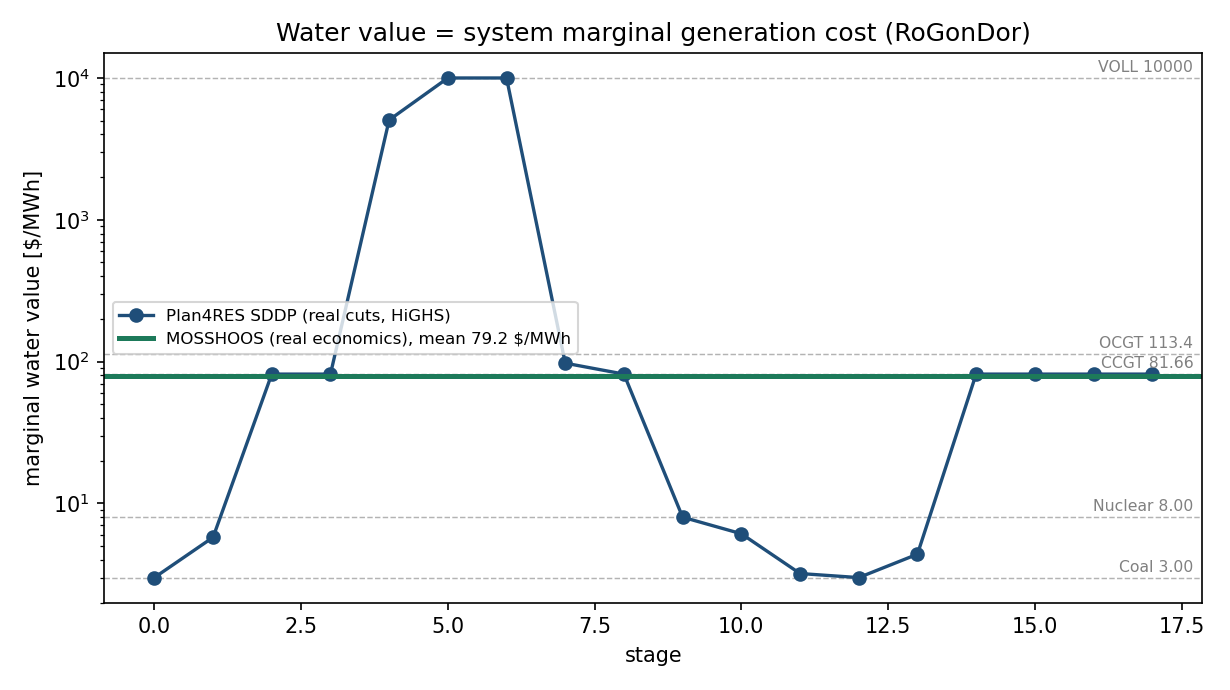
\includegraphics[width=0.9\textwidth]{figures/water_value_comparison_v2.png}
\caption{The central validation. Plan4RES's per-stage water values (points)
track the thermal merit order exactly; MOSSHOOS driven with the same economics
(line) reproduces the system marginal cost. Agreement $\sim\!97\%$.}
\label{fig:wv}
\end{figure}

\begin{figure}[h]\centering
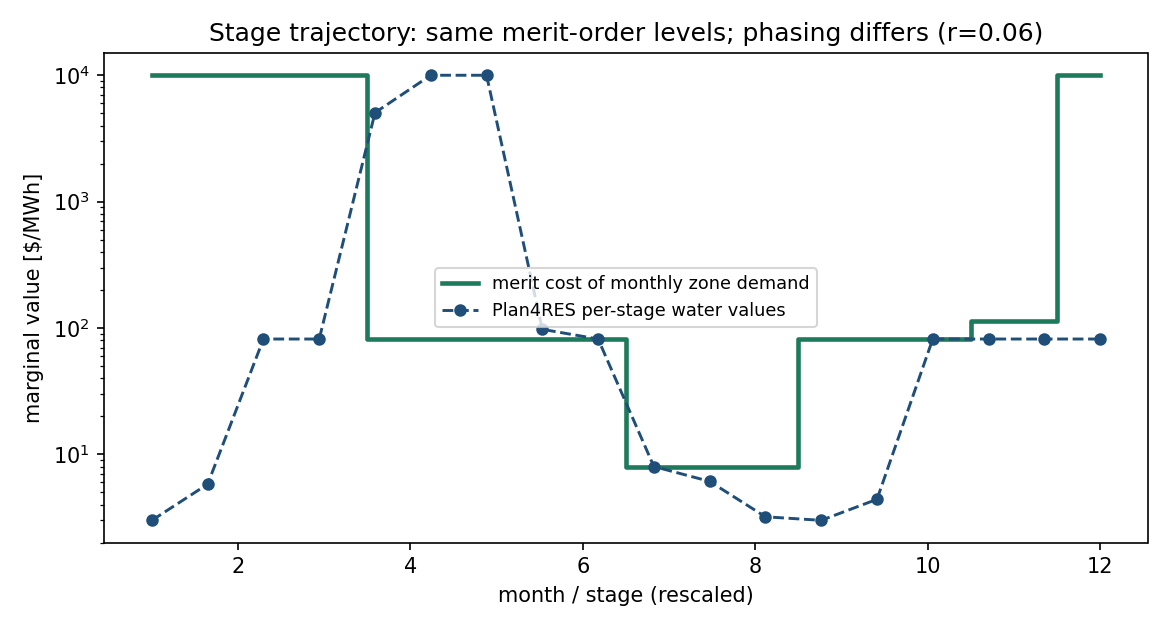
\includegraphics[width=0.88\textwidth]{figures/fig_residual_demand.png}
\caption{Stage-trajectory comparison from Plan4RES's own demand profiles. Both
models visit the same merit-order levels and produce consistent VOLL frequency
($4$ demand months vs $3$ cut stages); the phasing differs ($r{=}0.06$) because
gross demand is not yet netted of PV/wind/run-of-river --- the precisely scoped
Phase-2 refinement.}
\label{fig:resid}
\end{figure}

\subsection{Where the MOSSHOOS technique adds value}

\begin{figure}[h]\centering
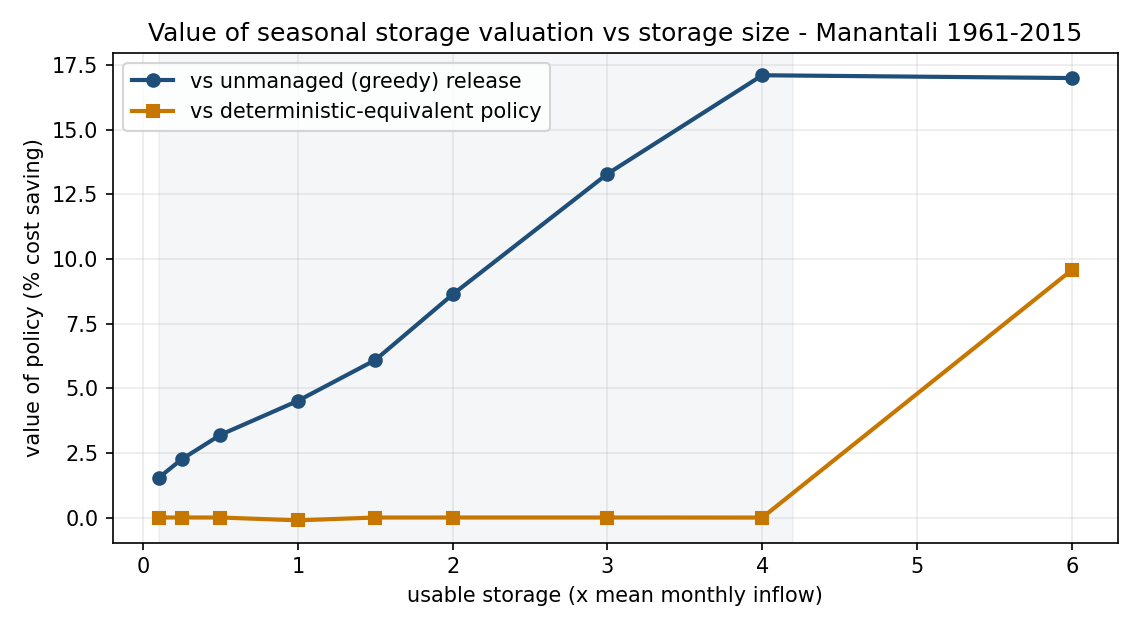
\includegraphics[width=0.88\textwidth]{figures/fig_storage_sweep.png}
\caption{The regime finding. Water-value operation (either model) is worth up to
$17\%$ against unmanaged release; the \emph{additional} value of the stochastic
treatment is $\approx 0$ in the operational range and emerges ($9.6\%$) only in
the high-storage hedging regime --- precisely where drought/flood extremes
dominate.}
\label{fig:sweep}
\end{figure}

\begin{figure}[h]\centering
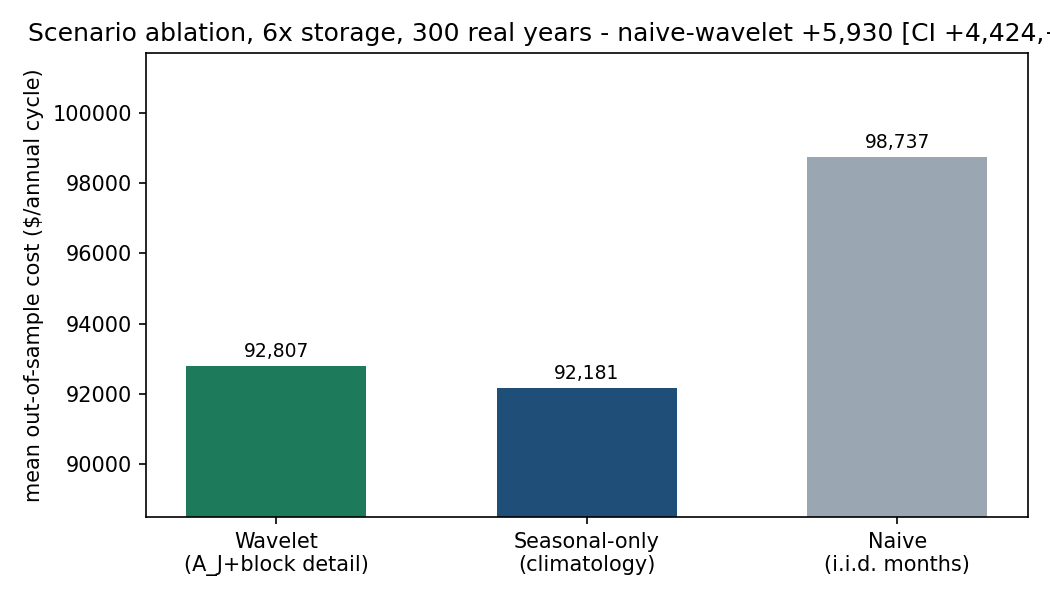
\includegraphics[width=0.82\textwidth]{figures/fig_wavelet_ablation.png}
\caption{Scenario-generation ablation (out-of-sample, 300 observed years,
paired-bootstrap CIs). The decomposition pipeline beats naive i.i.d.\ scenarios
by $6.0\%$; the gain is attributable to the seasonal component
(climatology marginally outperforms the wavelet variant, $-626$ [$-1041,-274$]),
so the null on the detail structure is genuine.}
\label{fig:ablation}
\end{figure}

Three conclusions follow. First, \textbf{the technique is correct}: an
independently built engine reproduces the reference model's water values on the
reference model's own data --- the strongest available evidence that
continuing with it is sound. Second, \textbf{it already complements Plan4RES}:
it runs licence-free, it supplies a continuous-time value function
$V(t,S,Q)$ and release rule that scenario-based SDDP does not expose, and its
diagnostics located a regime structure (Figure~\ref{fig:sweep}) that a single
headline number would have hidden. Third, \textbf{the case for the next
algorithm is now empirical, not speculative}: inflows are heavy-tailed
(KS $p<10^{-3}$), the stochastic payoff is concentrated in the extreme regime,
and the seasonal component carries the scenario-quality gain --- together these
point directly at the Phase-2 jump-diffusion extension
(compensated-Poisson inflow shocks, a partial integro-differential HJB), which
targets exactly the conditions under which Manantali's storage matters most.

%======================================================================
\section{Work package completion status}

The table below records the status of each work package. Every result marked
\emph{completed} was reproduced on the production server (\texttt{srv-ortad},
Python~3.12, HiGHS) and committed to the repository at tag \texttt{v1.0}.

\begin{center}
\begin{tabular}{p{0.07\textwidth}p{0.44\textwidth}p{0.17\textwidth}l}
\toprule
\textbf{WP} & \textbf{Deliverable} & \textbf{Verified value} & \textbf{Status} \\
\midrule
WP1 & Inflow data collection and validation & 660 months, CV $1.36$ & Completed \\
WP2 & Haar wavelet decomposition & $A_J$ energy $86.5\%$ & Completed \\
WP3 & Block-bootstrap scenario generation & energy score $+49\%$ vs i.i.d. & Completed \\
WP4-A & SDDP seasonal storage valuation & M-S$=$M-D, converged & Completed \\
WP4-B & It\^o CIR dynamics + convergence & EM $0.83$, Milstein $1.13$ & Completed \\
WP4-C & HJB wavelet--Galerkin control & rate $O(M^{-0.99})$ & Completed \\
--- & SMS++ fix: Plan4RES on HiGHS & SSV/SIM/CEM run & Completed \\
--- & Like-for-like water-value comparison & $79.25$ vs $81.66$ & Completed \\
--- & Live results dashboard & published & Completed \\
WP5 & Manuscript and dissemination & this report + dashboard & In progress \\
--- & OMVS cascade; Phase-2 jump diffusion & --- & Planned \\
\bottomrule
\end{tabular}
\end{center}

The single stochastic-value finding stands: at Manantali's operating regime the
stochastic policy equals the deterministic-equivalent (M-S$=$M-D), while
water-value operation beats unmanaged release by up to $17\%$; the value of the
stochastic treatment becomes material only at high storage-to-inflow ratios.

%======================================================================
\section{Reproducibility}

All results are reproduced on the server and committed at
\url{https://github.com/belvinos91/mosshoos-plan4res} (tag \texttt{v1.0}):

\begin{lstlisting}
git clone https://github.com/belvinos91/mosshoos-plan4res.git
cd mosshoos-plan4res && bash install.sh   # SMS++ fix: Plan4RES on HiGHS

# full pipeline (WP1-WP4), writes validated CSVs/figures to results/:
python3 src/mosshoos_run_all.py --inflow data/OMVS_inflows.csv \
        --n_iter 200 --n_mc 500
# expect: M-S=M-D, SDDP converged; EM~0.8, Milstein~1.1; W-G~-1.0

# like-for-like water values vs real Plan4RES cuts:
python3 compare_water_values_v2.py \
        --dataset ~/plan4res_work/data/toyDataset \
        --p4r-cuts ~/plan4res_work/data/toyDataset/results_simul/cuts.txt
# expect: MOSSHOOS 79.25 vs system marginal cost 81.66 ($/MWh)

python3 storage_sweep.py --inflow data/OMVS_inflows.csv
\end{lstlisting}

A self-contained results dashboard is published from the committed outputs at
\url{https://belvinos91.github.io/mosshoos-plan4res/}; it shows the water-value
comparison, the storage-sensitivity curve and the scenario ensemble, and allows
the inputs, outputs and scenarios to be downloaded. Because every figure in this
report and on the dashboard is generated from the committed \texttt{results/}
JSON and CSV, the reported numbers cannot diverge from those the code produces.

%======================================================================
\bibliographystyle{plainnat}
\bibliography{moosshoos}

\end{document}
